\documentclass[UTF8]{ctexart}

\usepackage{subfiles}  

%下面的语句, 引入你的头部设置文件
\usepackage{C:/phpStorm_proj/02_myself_ID_EGO/+100_latex_all_math_sel/myPreamble} 
%必须是绝对路径,才能让各个tex在单独编译时使用到

\title{文件名}


%---------------------------------


\begin{document}
	\tableofcontents % 生成目录
	\date{} % 若不写这句, 则默认也会渲染出日期, 所以我们要手动赋空值
	\maketitle  %这行代码, 让你前面的 title, author, date生效
	
	
	
	\part{条件概率}
	
	\section{``条件概率"的意思}
	
	条件概率是: 有A, B 两个事件, 和样本空间 Ω. 其中 $P(B) >0$, 则, 在B已经发生的条件下, A发生的概率, 就叫做A对B 的``条件概率". 记作:  P(A| 条件B), 读作``在B发生的条件下, A发生的概率”. \\
	
	即, 条件概率公式是: $
	P(A \ | condition B) =\dfrac{\overset{\text{这个分子即:\ AB同时发生了}}{\overbrace{\text{在B发生条件下,A发生的样本点数}}}}{\text{B里面有多少个样本点}}=\dfrac{\text{n}_{\text{AB}}}{\text{n}_{\text{B}}}
	$ \\
	
	还可写成:  $
	P(A \ | condition B) 
	=\dfrac{\text{P}\left( \text{A}\cap \text{B} \right)}{\text{P}\left( \text{B} \right)}
	=\dfrac{\frac{\text{n}_{\text{AB}}}{\text{n}}}{\dfrac{\text{n}_{\text{B}}}{\text{n}}}=\dfrac{\text{n}_{\text{AB}}}{\text{n}_{\text{B}}}
		$ \\
	
	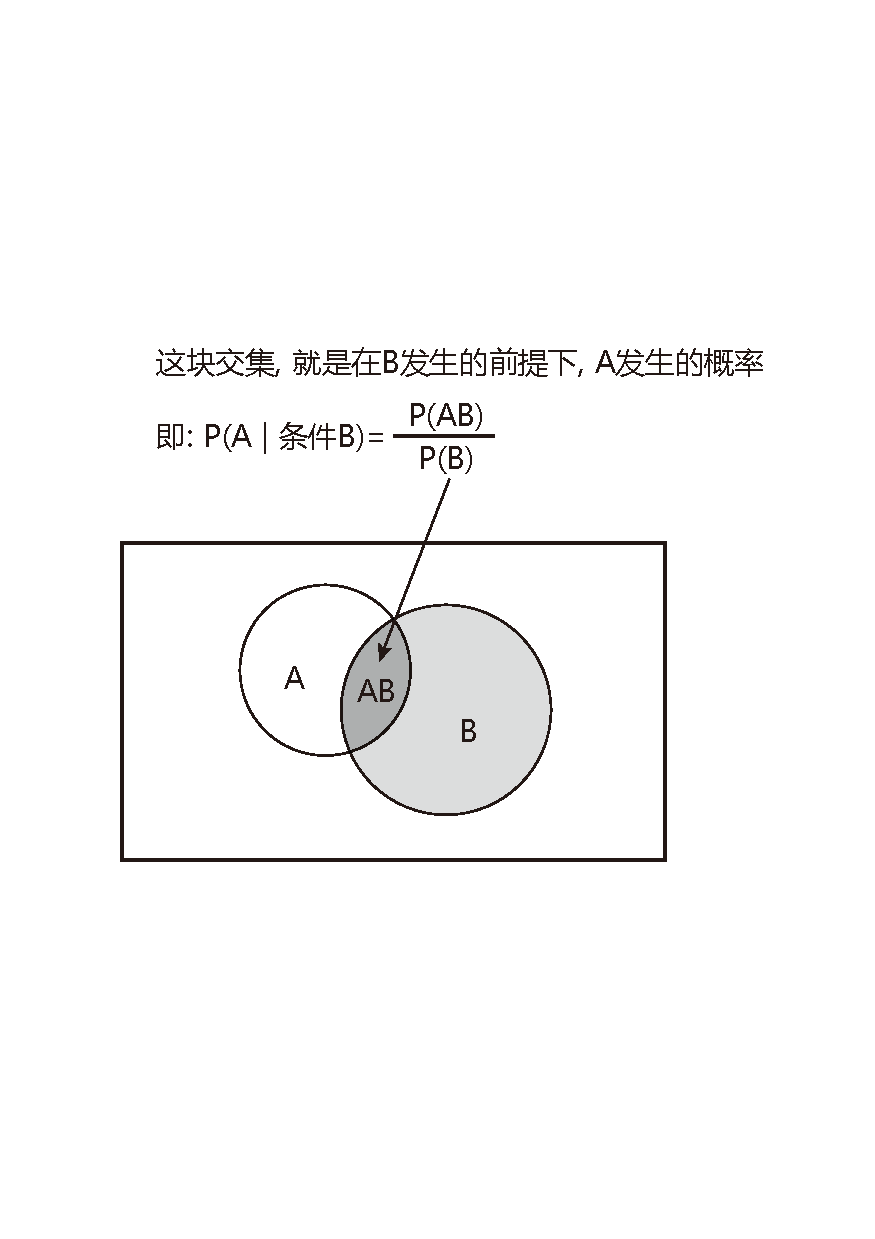
\includegraphics[width=0.5\textwidth]{/0088.pdf} \\
	
	如上图所示, 注意: 概率是个比值, 所以你光有分子那块的交集值, 是没用的, 它还需要与另一个数(分母)去比. \\
	
	上面公式中, P(AB) 的计算公式是什么呢? \\
	- 如果事件A, 和事件B 是相互独立的, 则 $P(AB) = P(A) \cdot P(B)$ \\
	- 如果事件A, 和事件B 不相互独立, 则只能用``条件概率"公式, 来求P(AB), 即: $P(AB) = P(A |B) \cdot P(B) = P(B |A) \cdot P(A) $   \\
	
	
	
	注意: ``条件概率", 和``分步骤法"的区别: \\
	- 分步骤法 (用乘法): 前后每一步骤的事件是相互独立的, 彼此没有条件关系.  \\
	比如, 第一步你结婚, 第二步我结婚. 我们这两件事发生的概率互不影响. \\
	
	- 条件概率 (里面也有用到乘法): 前面的事件, 有可能会(但并不一定)影响到后面事件的发生概率. 即前后事件之间并不互相独立.  \\
	会影响的例子: 比如一共有100个上岸机会, 则第一步你上岸的成功概率, 会影响到第二步我上岸的成功概率. (你若成功, 留给我的名额数量就会更少.) \\
	彼此独立的例子: 比如在你回国的条件下, 我出门的概率. 两者发生的概率毫无关系. 你回不回国, 跟我会出不出门没半毛钱关系.

		
	
	
	\begin{myEnvSample}
		有6个球, 各有编号.  我们先定义下这些事件: \\
		- B: 取到偶数编号的球 \\
		- $A_1$: 取到1号球 \\
		- $A_2$: 取到2号球 \\
		- $A_5$: 取到大于4号的球 \\
		
		则: \\
		- $
		\overset{\text{取到1号球的概率}}{\overbrace{\text{P(A}_1\text{)}}}=\frac{\overset{1\text{号球选}1}{\overbrace{\text{C}_{1}^{1}}}}{\underset{\text{全6选}1}{\underbrace{\text{C}_{6}^{1}}}}=\frac{1}{6}=0.166667
		$
		
		- $
		\text{P}\left( \text{A}_1|\text{B} \right) =\frac{\text{在B条件里面,取到A}_1\text{(即1号球)}}{\text{B:\ 取到偶数编号的球}}=\frac{\overset{\text{偶数编号的球里面,\ 取不到奇数编号的球}}{\overbrace{0}}}{\underset{3\text{个偶数球里面取1个}}{\underbrace{\text{C}_{3}^{1}}}}=0
		$
		
		- $
		\text{P}\left( \text{A}_2|\text{B} \right) =\frac{\overset{1\text{个编号2的球里面,取1个}}{\overbrace{\text{C}_{1}^{1}}}}{\underset{3\text{个偶数球里面取1个}}{\underbrace{\text{C}_{6}^{3}}}}=\frac{1}{3}
		$
		
		- $
		\text{P}\left( \text{A}_5|\text{B} \right) =\frac{\text{在B条件里面,取到大于4号的球}}{\text{B:\ 取到偶数编号的球}}=\frac{\overset{5,6\text{号与偶数的交集,\ 只有6号一个球}}{\overbrace{1}}}{3}
		$
			
	\end{myEnvSample}
	
	

	
	\section{条件概率的性质}
	
	\subsection{性质: $ P(A | \text{条件}B) >= 0$}
	
	
	\subsection{性质: $ P(\Omega | \text{条件}B) = 1$}
	
	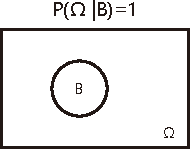
\includegraphics[width=0.25\textwidth]{/0089.pdf}
	
	
	\subsection{性质: $ \text{P}\left( \text{A}_1\cup \text{A}_2\ |\text{B} \right) =\text{P}\left( \text{A}_1\ |\text{B} \right) +\text{P}\left( \text{A}_2\ |\text{B} \right) -\text{P}\left( \text{A}_1\text{A}_2\ |\text{B} \right) 		$}
	
	\subsection{性质: $	\text{P}\left( \text{A\ |B} \right) =1-\text{P}\left( \overline{\text{A}}\ |\text{B} \right) 	$}
	
	\subsection{性质: 可列可加性:  若$ A_1, A_2, ... A_n, ...$ 是``互不相容"的事件, 则有: $ P(\sum_{i=1}^\infty A_i | B) = \sum_{i=1}^ \infty P(A_i | B)$ ← 即: ``和的概率", 等于``概率的和"} 
	
	
	
	
	
	
	
	\section{``条件概率"的乘法公式 : $ \boxed{			
		P(\text{前后})=P(\text{后}) \cdot P(\text{前}|\text{\text{后}}) = P(\text{\text{前}}) \cdot P(\text{后}|\text{前})}$}

	推导过程: \\
	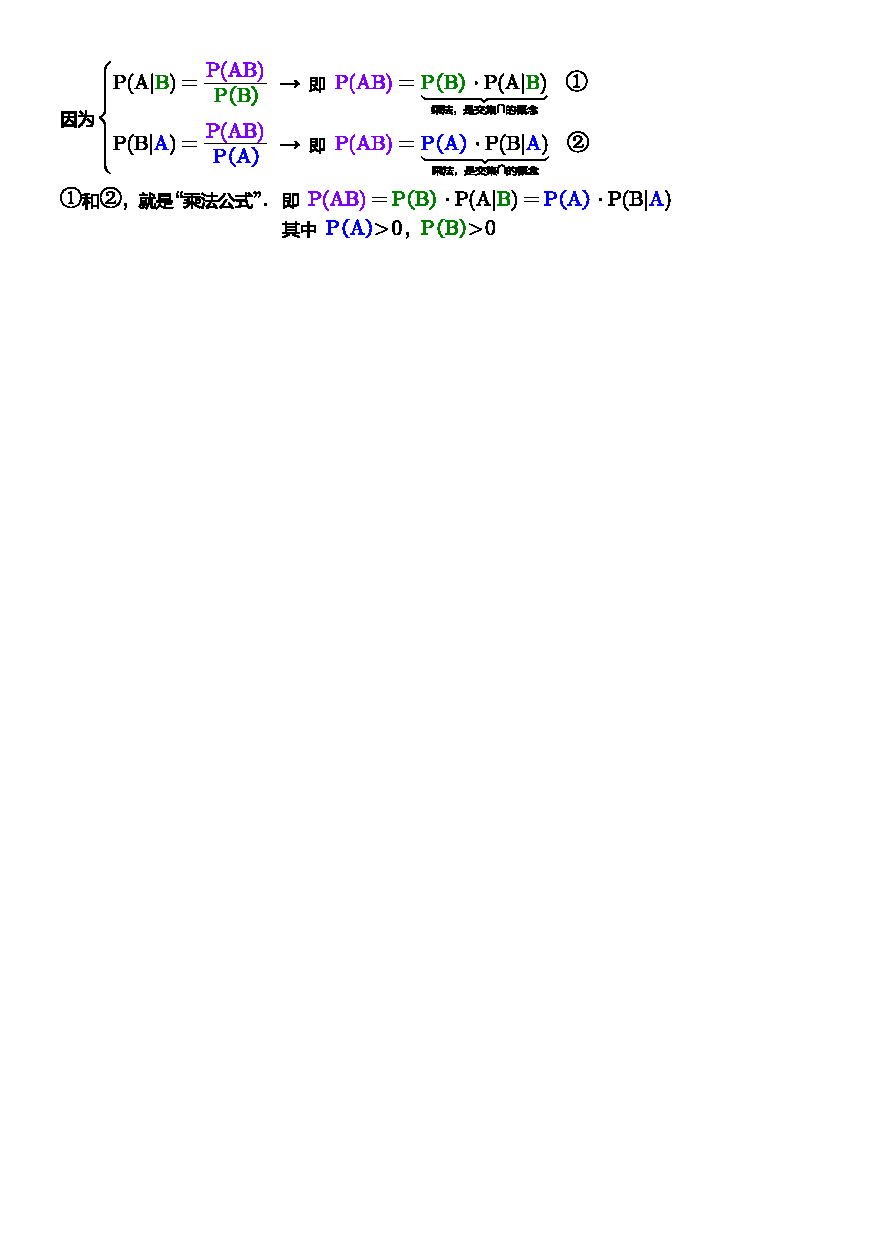
\includegraphics[width=0.8\textwidth]{/0090.pdf} \\
	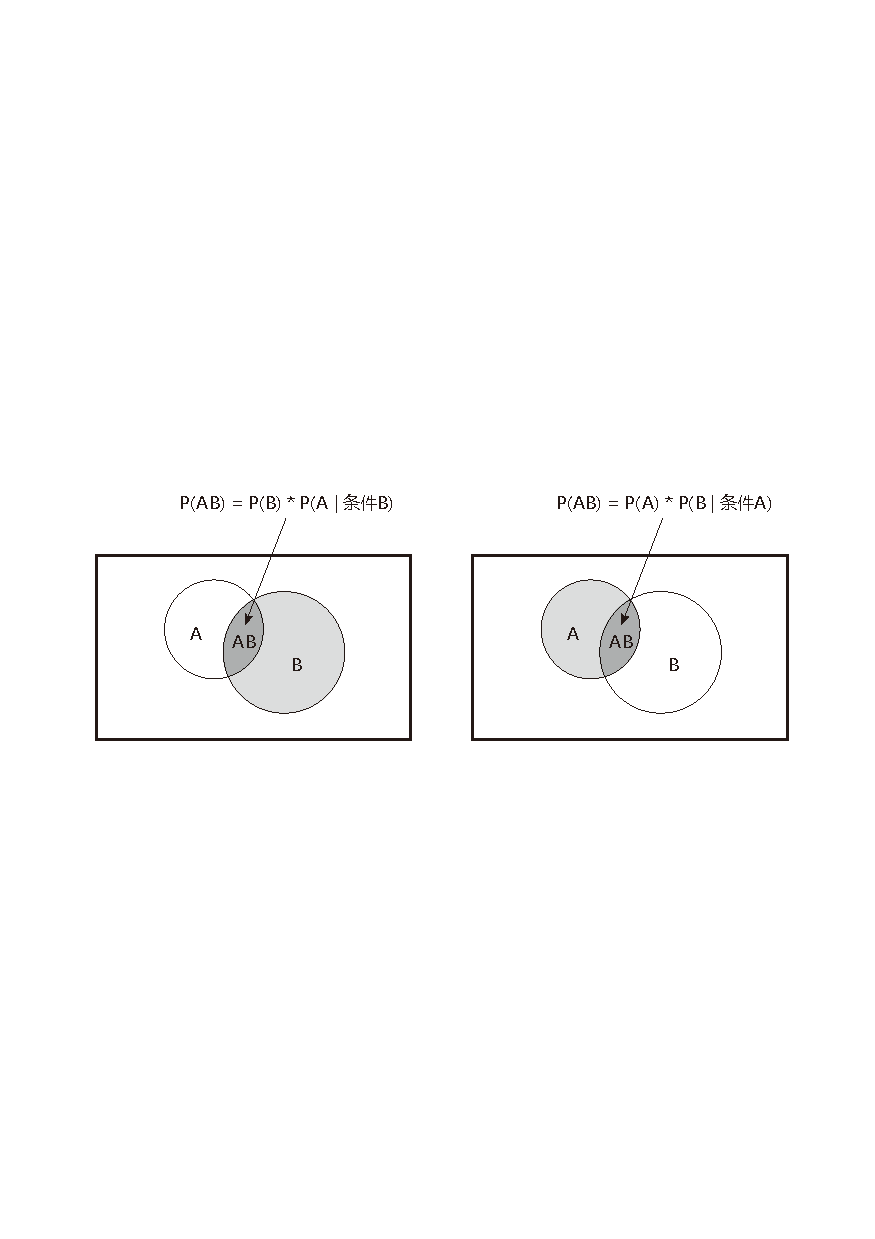
\includegraphics[width=0.8\textwidth]{/0091.pdf} \\
	
	同理, 多个事件的乘法公式就是:  \\
	→ $ \boxed{
	\text{P(ABC)}=\underbrace{\text{P(A)}}\cdot \underbrace{\text{P(B|A)}}\cdot \underbrace{\text{P(C|BA)}} 	
	}
	$ \\
	↑ 上面``从右往左"看, 就是按 A,B,C 的顺序 \\
	
	→ 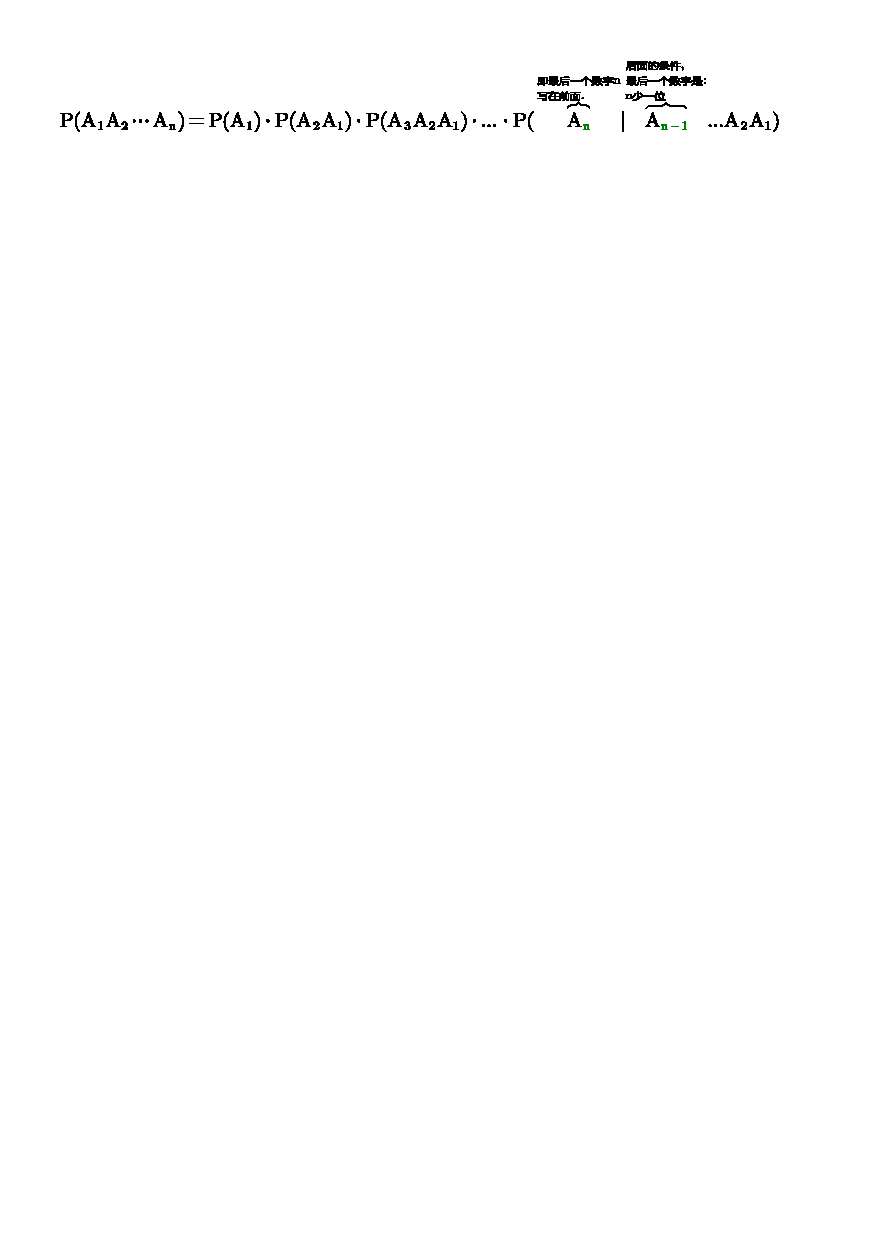
\includegraphics[width=0.95\textwidth]{/0092.pdf} \\
	↑ 上面``从右往左"看, 就是按$A_1, A_2, ... , A_n$的顺序 \\
	
	
	
	
	\begin{myEnvSample}
		有100件产品, 次品率=10\%, 即有10件次品. 做不放回抽样, 问: 第3次才取到合格品的概率是? \\
		我们先令: \\
		- $A_1$ 表示第1次取, 就取到了合格品 \\
		- $A_2$ 表示第2次取, 取到了合格品 \\
		- $A_3$ 表示第3次取, 取到了合格品 \\
		
		那么第3次才取到合格品, 就是:  \\
		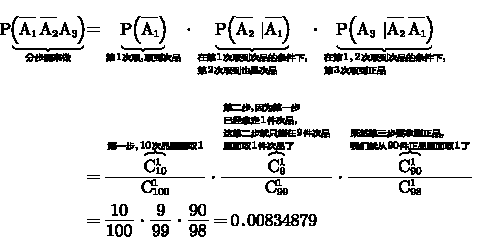
\includegraphics[width=0.8\textwidth]{/0093.pdf} 		
	\end{myEnvSample}
	
	


\begin{myEnvSample}
	某产品:  \\
	- 甲公司占60\%市场份额, 且其产品合格率是 90\% \\
	- 乙公司占40\%市场份额, 且其产品合格率是 80\% \\
	
	我们先定义下这些事件: \\
	- J: 表示产品是甲的 \\
	- $\overline{\text{J}}$: 表示产品是乙的 \\
	- Q (qualified) : 表示产品是``合格"的 \\
	- $\overline{\text{Q}}$ : 表示产品是``不合格"的 \\
	
    问, 你买一个产品, 是甲公司的, 并且是合格的概率是? \\
    $
    \text{P}\left( \text{JQ} \right) =\underset{=0.6}{\underbrace{\text{P}\left( \text{J} \right) }}\cdot \underset{\text{甲的合格率}=0.9}{\underbrace{\text{P}\left( Q \ | J \right) }}=0.54
    $ \\
    
    问, 你买一个产品, 是乙公司的, 并且是合格的概率是? \\
    $
    \text{P}\left( \overline{\text{J}}\text{Q} \right) =\underset{=0.4}{\underbrace{\text{P}\left( \overline{\text{J}} \right) }}\cdot \underset{\text{乙条件下的合格率}=0.8}{\underbrace{\text{P}\left(Q \ | \overline{\text{J}} \right) }}=0.32
    $      
\end{myEnvSample}





\begin{myEnvSample}
	抽签, 共10签, 其中有4个为``成功上岸"的好签. 甲乙丙三人, 按顺序依次去抽, 不放回. \\
	我们先设定事件:  \\
	- A: 表示甲 抽到``成功" \\
	- B: 表示乙 抽到``成功" \\
	- C: 表示丙 抽到``成功" \\
	
	问, (1) 甲抽到``成功"的概率? 
	$
	\text{P}\left( \text{A} \right) =\dfrac{\text{C}_{4\text{好签}}^{1}}{\text{C}_{10\text{签}}^{1}}=\frac{4}{10}=0.4
	$ \\
	
	(2) 甲乙都抽到``成功"的概率?  
\begin{align*}  % 支持每行编号. 若不需要编号, 就用 align*环境
	&\text{P}\left( \text{AB} \right) =\underset{\text{第1步:甲先成功}}{\underbrace{\text{P}\left( \text{A} \right) }}\cdot \underset{\text{第2步:在甲成功的前提下,\ 乙再成功}}{\underbrace{P(B|A) }}\\
&=\frac{\overset{\text{甲先抽掉一张好签}}{\overbrace{\text{C}_{4\text{好签}}^{1}}}}{\text{C}_{10\text{签}}^{1}}\cdot \frac{\overset{\text{乙就只能从剩下的3张好签中来抽了}}{\overbrace{\text{C}_{4\text{好签}-1}^{1}}}}{\text{C}_{10\text{签}-1}^{1}}
=\frac{4}{10}\cdot \frac{3}{9}=0.133333
\end{align*}


(3) 甲失败, 乙成功 的概率? 
\begin{align*}  % 支持每行编号. 若不需要编号, 就用 align*环境
&P\left( \overline{A}B \right) =\underset{\text{第1步:甲先失败}}{\underbrace{P\left( \overline{A} \right) }}\cdot \underset{\text{第2步:在甲失败的前提下,\,\,乙再成功}}{\underbrace{P\left( B\,\,|\overline{A} \right) }} \\
&=\frac{\overset{\text{甲先从共6张坏签中取}1}{\overbrace{\text{C}_{6\text{坏签}}^{1}}}}{\text{C}_{10\text{签}}^{1}}\cdot \frac{\overset{\text{乙从共4张好签中取}1}{\overbrace{\text{C}_{4\text{好签}}^{1}}}}{\text{C}_{10\text{签}-1}^{1}}=\frac{6}{10}\cdot \frac{4}{9}=0.266667
\end{align*}



(4) 甲乙丙都抽到``成功"的概率? 
\begin{align*}  % 支持每行编号. 若不需要编号, 就用 align*环境
	&P\left( ABC \right) =\underset{\text{第1步:甲先成功}}{\underbrace{P\left( A \right) }}\cdot \underset{\text{第2步:在甲成功的前提下,\,\,乙再成功}}{\underbrace{P\left( B\,\,|A \right) }}\cdot \underset{\text{第3步:在甲乙都成功的前提下,丙再成功}}{\underbrace{P\left( C|BA \right) }}\\
&=\frac{\text{C}_{4\text{好签}}^{1}}{\text{C}_{10\text{签}}^{1}}\cdot \frac{\text{C}_{\text{还剩3好签}}^{1}}{\text{C}_{\text{还剩9签}}^{1}}\cdot \frac{\text{C}_{\text{还剩2好签}}^{1}}{\text{C}_{\text{还剩8签}}^{1}}\\
&=\frac{4}{10}\cdot \frac{3}{9}\cdot \frac{2}{8}=0.0333333
\end{align*}
\end{myEnvSample}



	

\begin{myEnvSample}
	你的新邻居, 是个 is very shy and withdrawn, invariably helpful but with very little interest in people or in the world of reality. A meek and tidy soul, he has a need for order and structure, ant a passion for detail. \\
	你觉得他更可能是 -- 图书管理员, 还是农民? \\
	大多数人会认为他是图书馆管理员. 其实, 这种判断是"非理性"的. 问题的关键在于 -- 你没有把这两种职业的"人数比例"考虑进去. \\
	
	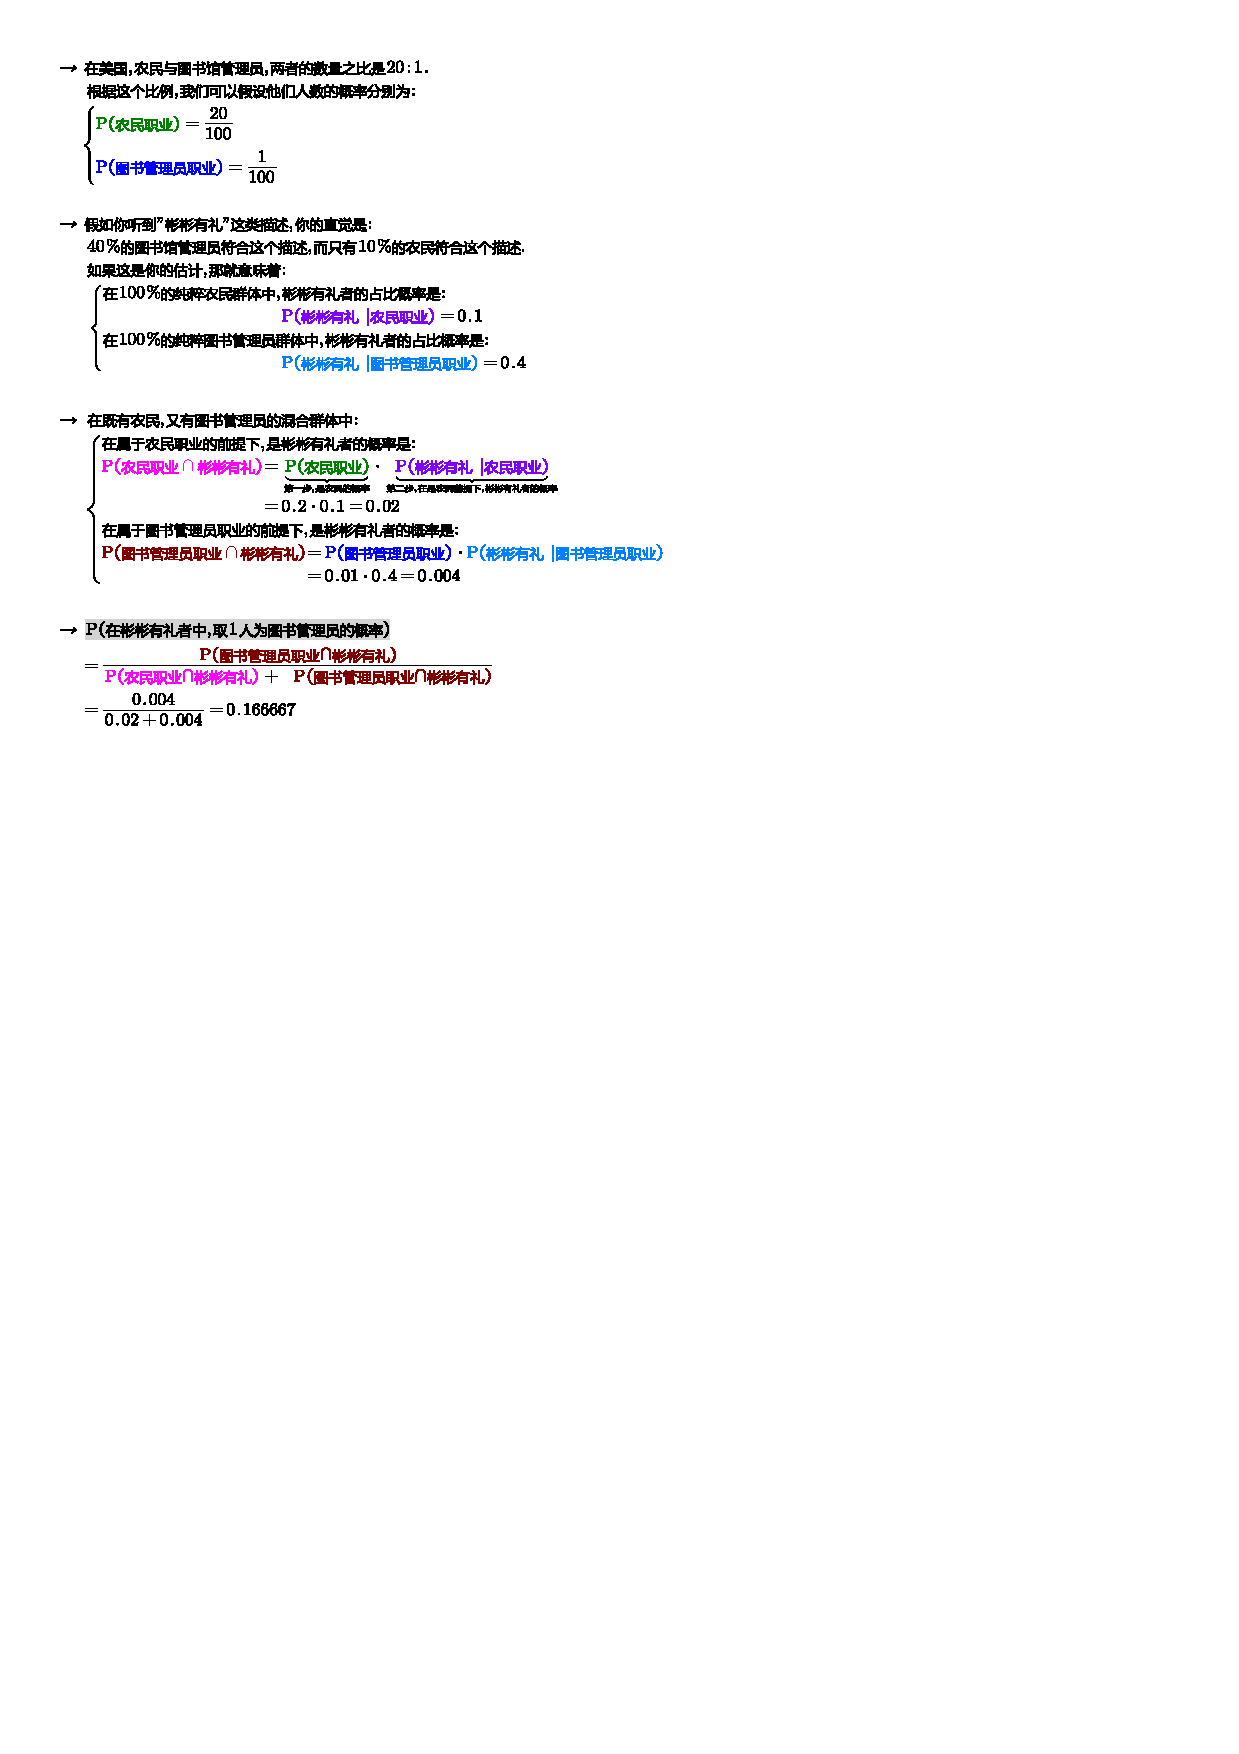
\includegraphics[width=1\textwidth]{/0099.pdf}
	
	所以, 即使你认为``符合这个描述的人是一个图书馆管理员的可能性, 是一个农民的4倍", 也抵不过农民的数量很多.
\end{myEnvSample}




\begin{myEnvSample}
	辛普森杀妻案, 原告证明辛普森常常家暴前妻. 他们认为, 长期家暴说明辛普森有杀妻的动机. 被告律师则举出数据反驳说, 美国有400万被家暴的妻子, 但只有1432名被丈夫杀害, 这个概率只有$ \frac{1432} {400\text{万}}$ = 比1/2500还低. 所以家暴证明不了辛普森谋杀. \\	
	被告想表达的是: 在``家暴"这个事件前提条件下, 丈夫谋杀妻子的概率不高. 即 P(丈夫家暴∩丈夫杀妻) = 概率值很低.  \\
	
	你怎么看? 事实上, 被告举出的概率, 不适用于这个案子上. 因为本案的妻子已经死亡, ``妻子已死"也变成了一个已经存在的前提条件. 所以现在我们要看的概率就是:  P(丈夫家暴∩妻子已死亡∩是丈夫杀妻)=?  即: 在``被家暴"且``死亡"的妻子数量里面 (这里就有两个前提条件了, 而不是仅一个前提条件), 有多少是被丈夫杀害的?  \\
	
	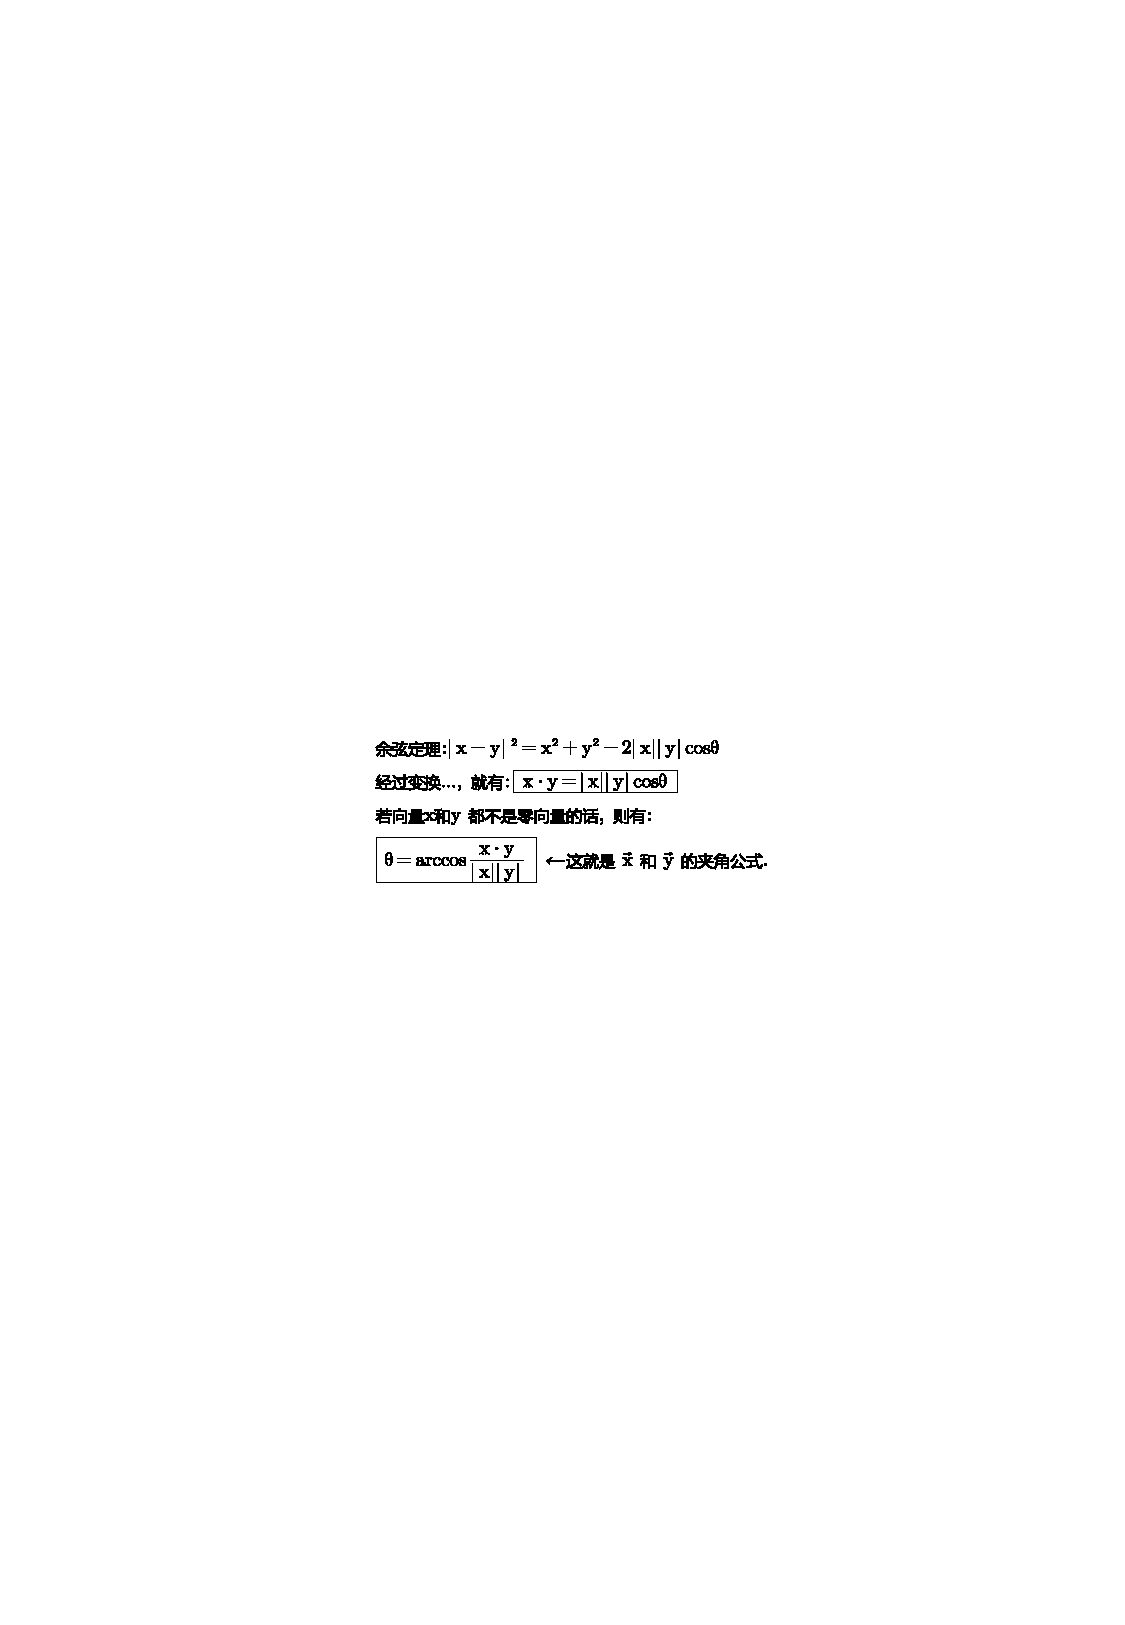
\includegraphics[width=0.6\textwidth]{/0100.pdf} \\
	即: \\
	- 辛普森律师一方 的概率公式是: $ \dfrac{\text{红色}} {Violence} < \frac{1} {2500}$ \\
	- 妻子一方律师 的概率公式是: $ \dfrac{\text{红色}} {\text{红色+黄色}}=93\% $ \\
	
	
	根据美国1992年发布的数据推算: 每10万个被家暴的妇女中, 有43个会被谋杀. 其中40个是被丈夫谋杀, 其他3个是被丈夫以外的人谋杀. 那么, 条件概率就是: \\
	$
	P\left( A\ |B \right) =\frac{P\left( AB \right)}{P\left( B \right)}
	$ \\
	$
	P\left( \text{丈夫杀\ |家暴}\cap \text{妻死} \right) =\dfrac{P\left( \text{家暴}\cap \text{妻死}\cap \text{丈夫杀} \right)}{P\left( \text{家暴}\cap \text{妻死} \right)}=\dfrac{\dfrac{40}{100000}}{\dfrac{43}{100000}}=0.930233
	$\\
	
	你仔细体会一下两者的不同: \\
	- 辛普森方, 是说: 在所有``之后活着和死去"的被家暴的妻子里, 被丈夫杀了的可能性是多大. 即 $\dfrac{\text{丈夫杀害}} {\text{条件: 1.被家暴}}$ \\
	- 妻子方, 是说: 在所有``死去"的被家暴的妻子里, 被丈夫杀了的可能性是多大? 即$ \dfrac{\text{\text{丈夫杀害}}} {\text{条件: 1.被家暴 \& 2.死亡}}$ \\
	
	不过, 即使概率高达93\%,也不能绝对证明辛普森杀了妻子. 因为\textbf{``条件概率"只表示统计意义上的``相关性", 并不代表``因果关系".} 即只说明: 家暴和谋杀妻子之间有很强的相关性。
	
	
\end{myEnvSample}









\section{传染病模型}


\begin{myEnvSample}
	有红球a个, 黑球b个. 你从中取出一个球, 看到其颜色后, 把它放回, 并同时再放入c个与你看到的颜色相同的球. 	问:  连续3次都是取出红球的概率? \\
	先设定事件: \\
	- $A_1$ : 表示你第1次, 取出的是红球 \\
	- $A_2$ : 表示你第1次, 取出的是红球 \\	
	- $A_3$ : 表示你第3次, 取出的是红球 \\	
	
	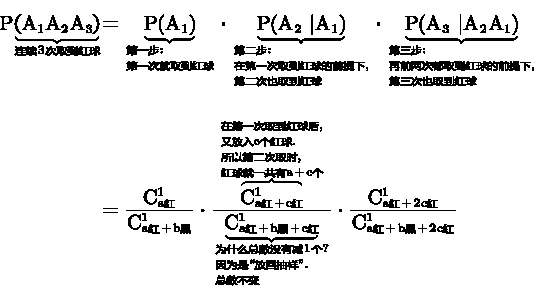
\includegraphics[width=0.85\textwidth]{/0094.pdf} \\
	
	上面可以看出: \\
	- 当 c红= 0 时, 就是正常的``放回抽样". \\
	- 当 c红= -1 时, 就是``不放回抽样". 即把之前步骤中取到的球, 拿走了, 不放回总体中. \\
	- 当 c红>0 时, 就是本例的``传染病模型".	
\end{myEnvSample}



~\\
\hrule
~\\

	
	\section{全概率公式 : $
		P\left( B \right) =\underbrace{P\left( A_1 \right) \cdot P\left( B|A_1 \right) }+\underbrace{P\left( A_2 \right) \cdot P\left( B|A_2 \right) }+...+\underbrace{P\left( A_n \right) \cdot P\left( B|A_n \right) }
		$}
	
	全概率公式 Total Probability Theorem: \\	
	如果 $A_1, A_2, ..., A_n$ 构成一个``完备事件组", 即: (1) 这些事件两两互不相容,  (2)其``和"(或``并集")为全集 $\Omega$, (3) $P(A_i)>0$. \\
		
	则有:
$\boxed{
\sum_{i=1}^n{\,\,\left[ P\left( A_i \right) \cdot P\left( B|A_i \right) \right]}=P\left( B \right) 
}
$ \\


即有: $
P\left( B \right) =\underbrace{P\left( A_1 \right) \cdot P\left( B|A_1 \right) }+\underbrace{P\left( A_2 \right) \cdot P\left( B|A_2 \right) }+...+\underbrace{P\left( A_n \right) \cdot P\left( B|A_n \right) }
$ \\

	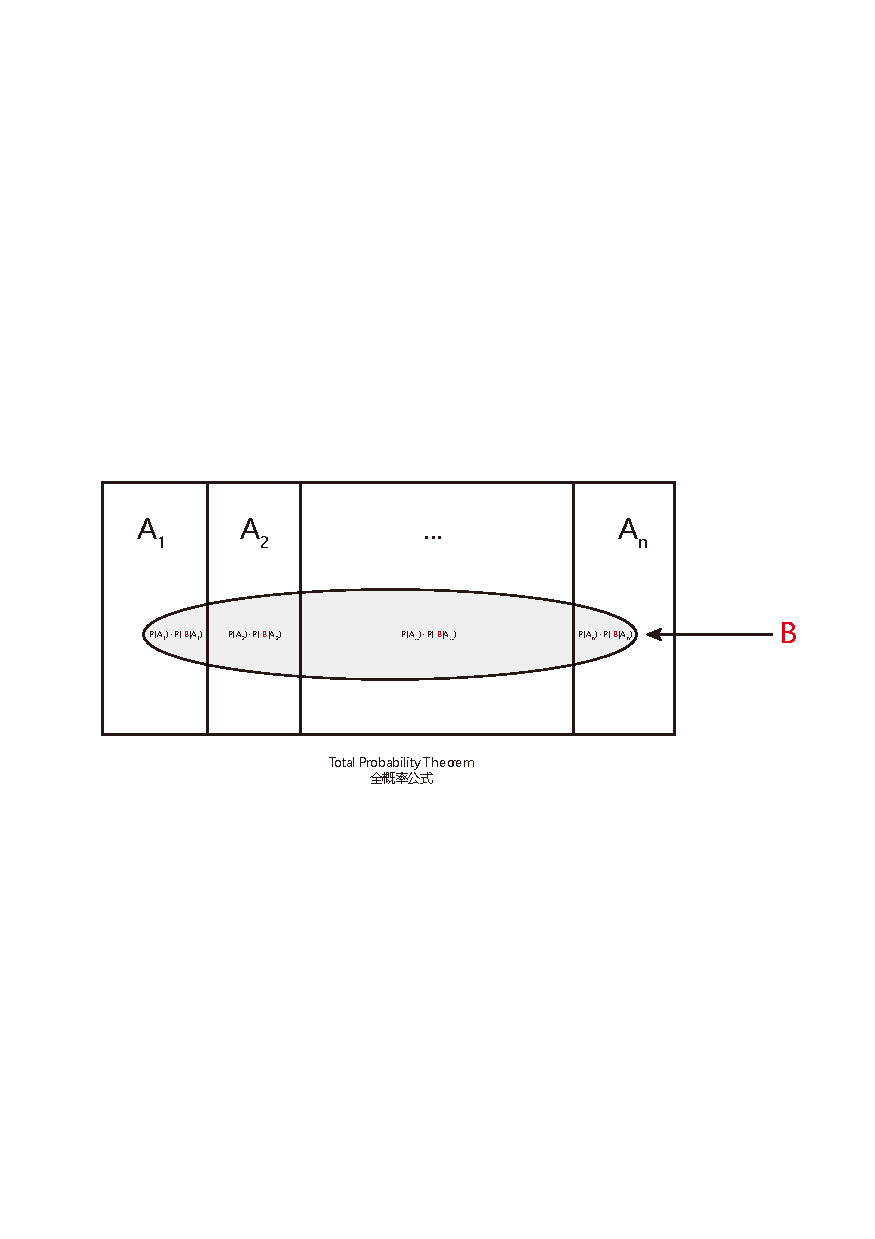
\includegraphics[width=1\textwidth]{/0095.pdf}
	
	
	\begin{myEnvSample}
		一个工厂, 有4条生产线, 情况如下: \\	
		\begin{tabular}{|l| l| l| l| l|}
			\hline
		 	&  生产线1  & 生产线2  &  生产线3 & 生产线4 \\
			\hline
			产量 &  15\% & 20\% & 30\% & 35\% \\
			\hline
			不合格率 &  0.05 & 0.04 & 0.03 & 0.02 \\
			\hline
		\end{tabular} \\
	
	问: 从该工厂的产品中, 任取一件, 是``不合格品"的概率? \\
	
	我们先设定事件: \\
	- $A_1$ : 表示是 生产线1 中的产品 \\
	- $A_2$ : 表示是 生产线2 中的产品 \\
	- $A_3$ : 表示是 生产线3 中的产品 \\
	- $A_4$ : 表示是 生产线4 中的产品 \\
	- $B$ : 表示是次品 \\
	
	那么, 你任取一件为不合格的概率, 不就是整个工厂总的不合格概率么?! 即 =P(B) \\		
		\begin{align*}
	&P\left( B \right)\\
&=\underset{\text{第1条生产线中}\left( \text{的条件下} \right) ,\,\,\text{不合格品的概率}}{\underbrace{\overset{\text{产品属于生产线1的概率}}{\overbrace{P\left( A_1 \right) }}\cdot \overset{\text{生产线1中的次品率}}{\overbrace{P\left( B|A_1 \right) }}}}+P\left( A_2 \right) \cdot P\left( B|A_2 \right) +P\left( A_3 \right) \cdot P\left( B|A_3 \right) +P\left( A_4 \right) \cdot P\left( B|A_4 \right)\\
&=(15\%\cdot 0.05)+(20\%\cdot 0.04)+(30\%\cdot 0.03)+(35\%\cdot 0.02)\\
&=0.0315
		\end{align*}
	\end{myEnvSample}



\begin{myEnvSample}
	有10台机器人, 3台是次品. 已经卖出去了2台(是正品还是次品未知). \\
	问: 再取1台, 是正品的概率? \\
	
	首先, 我们定义事件:  \\
	- $B_{00}$ : B(bad),  表示前两次取, 都是次品(用0表示) \\
	- $B_{10}$ : 表示前两次取, 是 一正(用1表示), 一次(用0表示). 至于顺序是``正,次" 还是``次,正", 都行 \\
	- $B_{11}$ : 表示前两次取, 都是正品 \\
	- $G_{xx3}$ : G(good),  表示第三次取, 是正品 \\
	
	那么, 第3次取到正品 $P(G_{xx3})$ 的情况, 就有这3种可能性: \\
	- (第1次取到)次, (第2次取到)次, (第4次取到)正.  \\
	即 → $=
	\underset{\text{前两次取到次品}}{\underbrace{\text{P}\left( \text{B}_{00} \right) }}\cdot \underset{\text{在前两次取到次品的条件下,\ 第3次取到正品}}{\underbrace{\text{P}\left( \text{G}_{\text{xx}3}\ |\text{B}_{00} \right) }}
	$ \\
	- 次,正,正.  即 → $=
	\text{P}\left( \text{B}_{10} \right) \cdot \text{P}\left( \text{G}_{\text{xx}3}\ |\text{B}_{10} \right) 
	$ \\
	- 正,正,正. 即 →  $=
	\text{P}\left( \text{B}_{11} \right) \cdot \text{P}\left( \text{G}_{\text{xx}3}\ |\text{B}_{11} \right) 
	$\\
	
	上面这三种可能性并存, 就是``和"(并集)的概念. 用加法: \\
	
	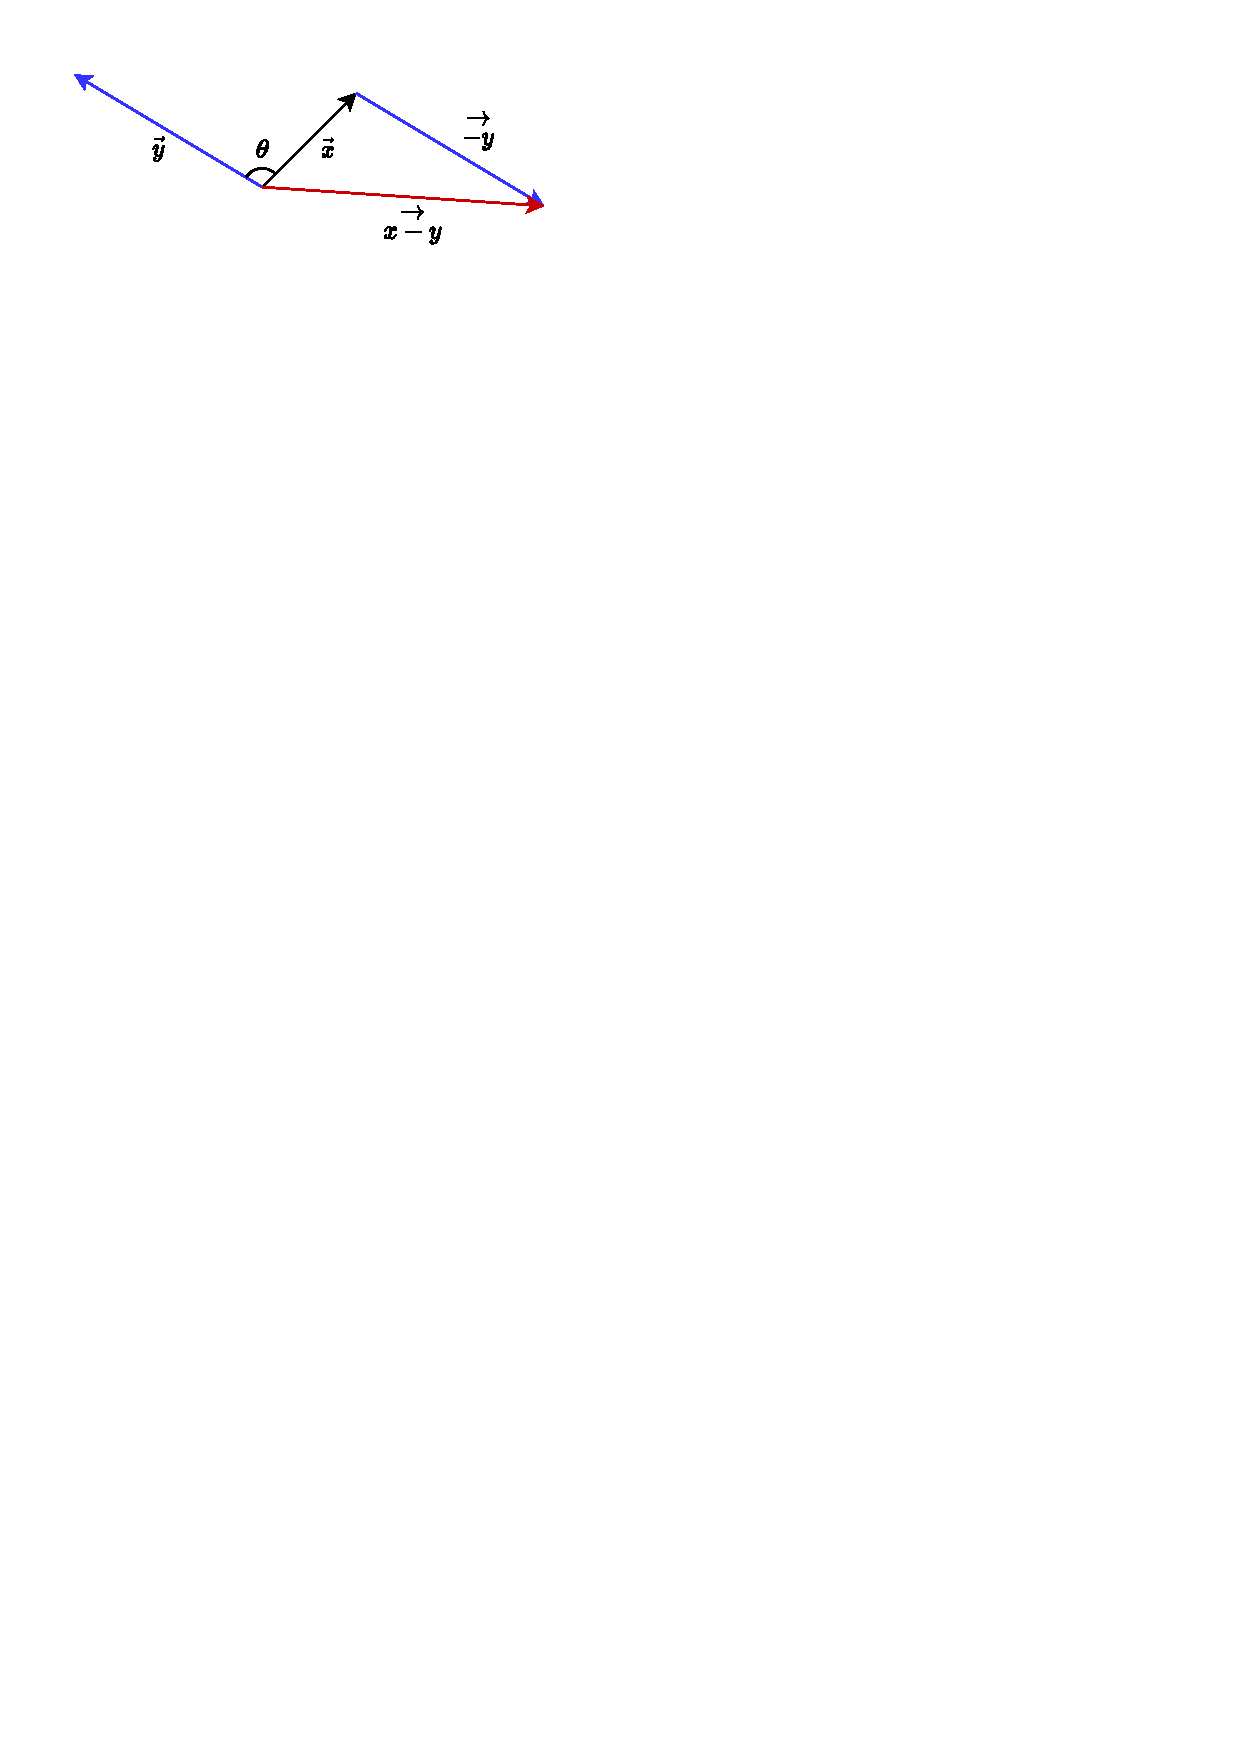
\includegraphics[width=1\textwidth]{/0096.pdf}
	
	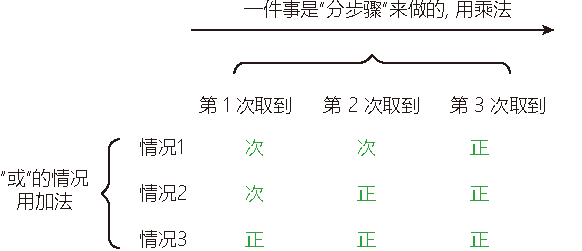
\includegraphics[width=0.7\textwidth]{/0097.pdf}
\end{myEnvSample}





\begin{myEnvSample}
	有10件产品, 其中次品的数量, 有三种可能性: 0件 /1件 /2件, 即这三种可能性中的每一种, 发生的概率是1/3.  \\
	同时, 检验时也存在``误检"情况 : \\
\begin{tabular}{|l|l|l|l|}
	\hline
	& →被检验成→ &    & 的概率是   \\
	\hline
	正品 &        & 次品 & 0.02    \\
	\hline
	正品 &    →    & 正品 & 0.98    \\
	\hline
	次品 &   →     & 正品 & 0.05    \\
	\hline
	次品 &        & 次品 & 0.96  \\
	\hline
\end{tabular}\\

	问: 这批产品能通过检验(即事件$S_2$)的可能性是多少? 即本题要求 P($S_2$)=? \\
	这要分两种情况来讨论 (``和"的概念, 用加法): \\
	- 1. 正品被误检(成``假")时的情况 \\
	- 2. 次品被误检(成``真")时的情况 \\
	
	我们先定义各种事件: \\
	- $B_0$ : B(bad). 表示总的10件产品中, 存在0件次品. 该事件的概率, 题目已经告诉我们: $\text{P}\left( \text{B}_0 \right) =\frac{1}{3}$
	\\
	- $B_1$ : 表示总的10件产品中, 存在1件次品. $\text{P}\left( \text{B}_1 \right) =\frac{1}{3}$
	\\
	- $B_2$ : 表示总的10件产品中, 存在2件次品. $\text{P}\left( \text{B}_2 \right) =\frac{1}{3}$
	\\
	- $S_1$ : S(sample. (v.) 抽样检验;取样;采样) 表示任意抽检一次, 抽到了正品. (但这里还有个问题不清晰, 就是说这个正品, 到底是它本身就是``正品"; 还是说只是抽验认为它是``正品"?) \\
	- $\overline{S_1}$ : 表示任意抽检一次, 抽到了次品. \\
	- $S_2$ : 表示再次检验, 并``通过验证" (注意: 有误检率存在. 所以通过检验的, 未必是``正品"; 反之亦然). \\
	
	
	本题要求的 P($S_2$), 实际上就是: ``无论第一次抽, 认为是正是次; 在第二次检验时, 都认为是正品"的东西. 即: $
	\text{P}\left( \text{S}_2 \right) =\underset{\text{第一次抽为正品,第二次检验为正}}{\underbrace{\text{P}\left( \text{S}_1 \right) \cdot \text{P}\left( \text{S}_2\ |\text{S}_1 \right) }}+\underset{\text{第一次抽为次品,第二次检验为正}}{\underbrace{\text{P}\left( \overline{\text{S}_1} \right) \cdot \text{P}\left( \text{S}_2\ |\overline{\text{S}_1} \right) }}
	$ \\
	
	那么我们先考算 $	\text{P}\left( \text{S}_1 \right) 	$ 和	$	\text{P}\left( \overline{\text{S}_1} \right) 	$. \\
	
	→ $	\text{P}\left( \text{S}_1 \right) 	$ : 是在具体``次品"数量未知的情况下, 抽1次就得到``正品"的概率. \\
	\begin{align*}  % 支持每行编号. 若不需要编号, 就用 align*环境
&	\text{P}\left( \text{S}_1 \right) =\underset{\text{在总数中有0次品的条件下,\ 抽1次得到正品的概率}}{\underbrace{\overset{\text{总数中有0次品}}{\overbrace{\text{P}\left( \text{B}_0 \right) }}\cdot \text{P}\left( \overset{\text{第1次抽得到正品}}{\overbrace{\text{S}_1}}|\text{B}_0 \right) }}+\underset{\text{总数中含有1次品,\ 抽1次取到正}}{\underbrace{\text{P}\left( \text{B}_1 \right) \cdot \text{P}\left( \text{S}_1|\text{B}_1 \right) }}+\underset{\text{总数中含有2次品,\ 抽1次取到正}}{\underbrace{\text{P}\left( \text{B}_2 \right) \cdot \text{P}\left( \text{S}_1|\text{B}_2 \right) }}\\
&=\underset{\text{总10中含有0次品}}{\underbrace{\frac{1}{3}\cdot \frac{\text{C}_{\text{总10正}}^{1}}{\text{C}_{\text{总}10}^{1}}}}+\underset{\text{总10中含有1次品}}{\underbrace{\frac{1}{3}\cdot \frac{\text{C}_{\text{总9正}}^{1}}{\text{C}_{\text{总}10}^{1}}}}+\underset{\text{总10中含有2次品}}{\underbrace{\frac{1}{3}\cdot \frac{\text{C}_{\text{总8正}}^{1}}{\text{C}_{\text{总}10}^{1}}}}\\
&=0.9  
	\end{align*} 	

	所以 : $
	\text{P}\left( \overline{\text{S}_1} \right) =1-\text{P}\left( \text{S}_1 \right) =1-0.9=0.1
	$ \\
	
	于是, 我们就能得到 : \\
	\begin{align*}  % 支持每行编号. 若不需要编号, 就用 align*环境
	&\text{P}\left( \text{S}_2 \right) =\underset{\text{第一次抽为正品,第二次检验为正}}{\underbrace{\overset{=0.9}{\overbrace{\text{P}\left( \text{S}_1 \right) }}\cdot \overset{\text{从上面的表格中可知,\ 正品被检验为正品,概率为}0.98}{\overbrace{\text{P}\left( \text{S}_2\ |\text{S}_1 \right) }}}}+\underset{\text{第一次抽为次品,第二次检验为正}}{\underbrace{\overset{=0.1}{\overbrace{\text{P}\left( \overline{\text{S}_1} \right) }}\cdot \overset{\text{次品被检验为正品,\ 概率是}0.05}{\overbrace{\text{P}\left( \text{S}_2\ |\overline{\text{S}_1} \right) }}}}\\
&=\left( 0.9\cdot 0.98 \right) +\left( 0.1\cdot 0.05 \right) =0.887\\
	\end{align*}

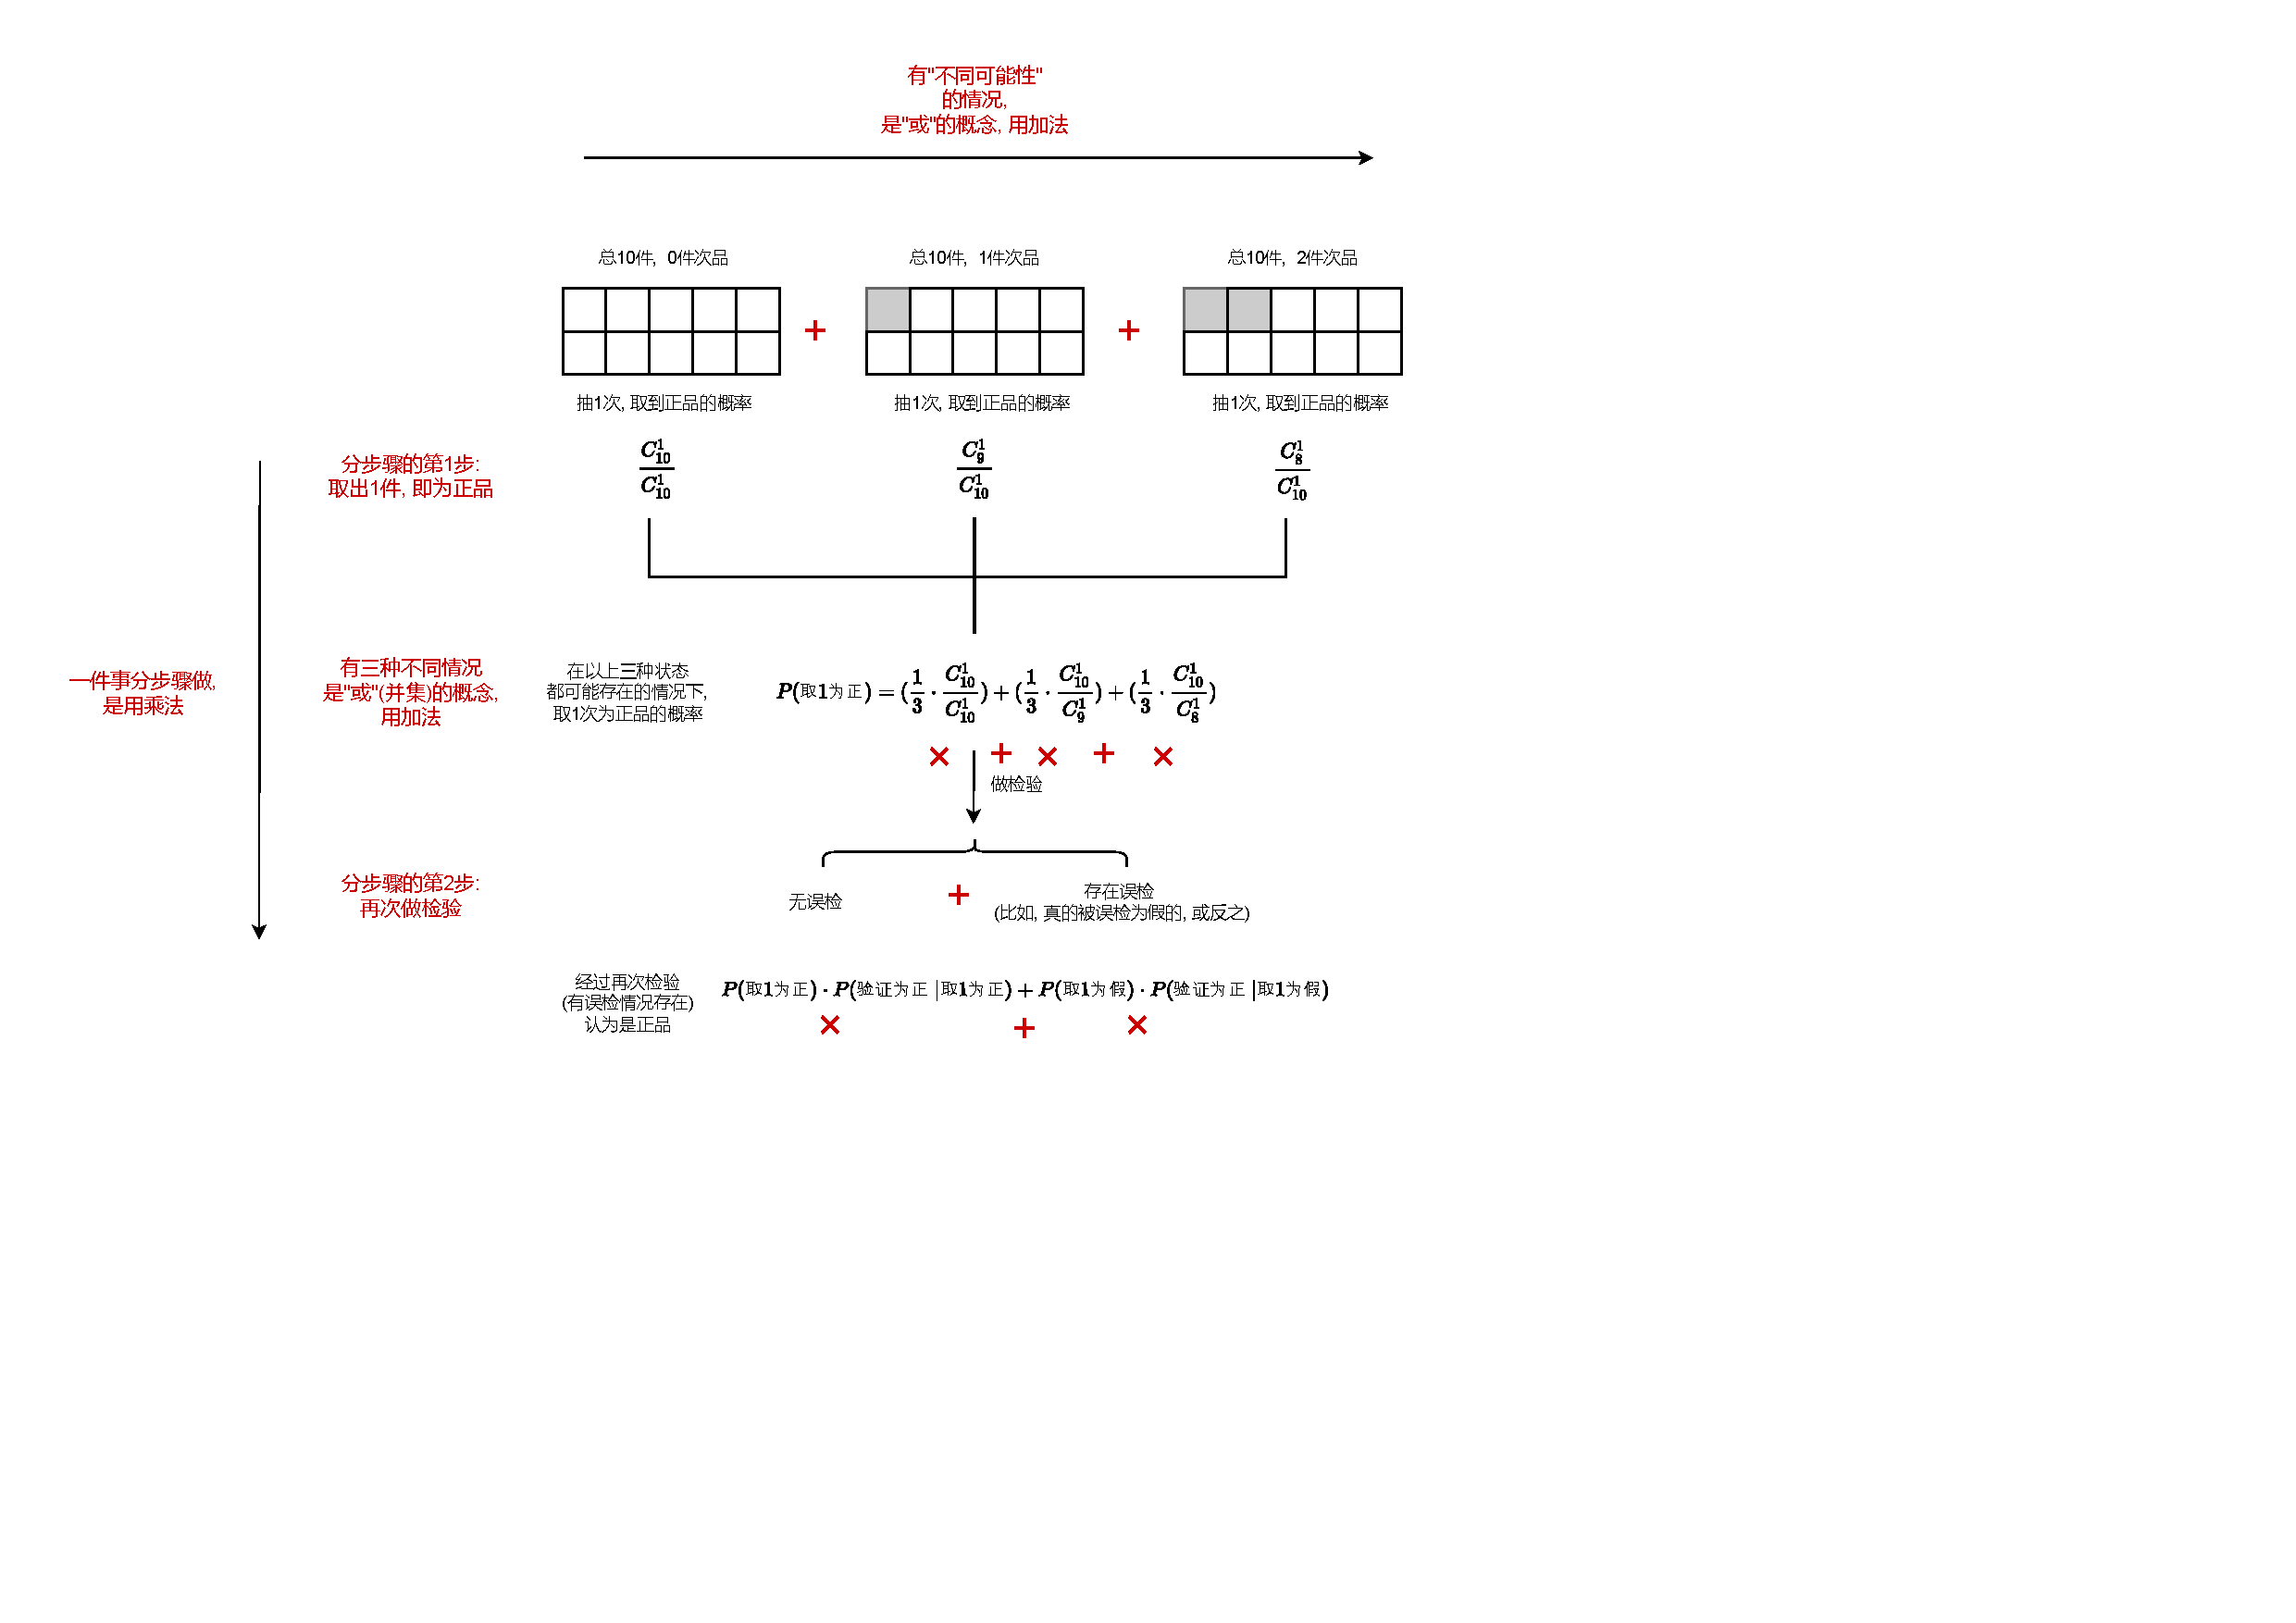
\includegraphics[width=1\textwidth]{/0098.pdf}
\end{myEnvSample}


~\\
\hrule
~\\



\section{贝叶斯公式 Bayes' theorem}

\subsection{先验概率 (从经验来推后果) \& 后验概率(更新迭代经验)}

\begin{tabular}{|p{0.6\textwidth}|p{0.4\textwidth}|}
	\hline
先验概率 :	是指根据以往经验和分析得到的概率,它往往作为``由因求果"问题中的``因"出现.  
&   
``先验概率"的计算比较简单,没有使用``贝叶斯公式". \\
	\hline
后验概率: 是基于新的信息,修正原来的``先验概率"后, 所获得的更接近实际情况的概率估计.	
& ``后验概率''的计算,要使用``贝叶斯公式".
	  \\
	\hline
\end{tabular}
























	
	
	
\end{document}